\chapter{Signal Efficiency}
\label{chap:eff}

The signal efficiency of finding displaced dilepton vertex is defined by the ratio of the number of events passing the signal selection (Chapter~\ref{chap:signal_selection}) to the total number of events processed. The signal efficiency can be written as Eq.~\ref{eq:OverallEff}. 

\begin{equation}
\label{eq:OverallEff}
\varepsilon_{\mathrm{overall}} = \varepsilon_{\mathrm{filter}} \cdot \varepsilon_{\mathrm{trigger}} \cdot 
                     (\varepsilon_{\mathrm{tracking}} \cdot \varepsilon_{\mathrm{lepton}})^2 \cdot
                     (\varepsilon_{\mathrm{vertexTrack}})^2 \cdot
                     \varepsilon_{\mathrm{vertexFit}}.
\end{equation}

$\varepsilon_{\mathrm{filter}}$ and $\varepsilon_{\mathrm{trigger}}$ together represent the efficiency of \texttt{RPVLL} filter, the ratio of the events passing \texttt{RPVLL} filter to the total events processed. \texttt{RPVLL} filter has the trigger filter as one of its requirements, and because it is desirable to study the trigger efficiency independently from the filter efficiency, \texttt{RPVLL} filter efficiency is factorized into the filter efficiency and the trigger efficiency. $\varepsilon_{\mathrm{tracking}}$ represents the efficiency to reconstruct ID tracks from signal particles, and $\varepsilon_{\mathrm{lepton}}$ represents the efficiency to reconstruct and identify the signal particles as leptons using ID tracks, energy deposite in calorimeters, and MS tracks. $\varepsilon_{\mathrm{vertexTrack}}$ represents the efficiency for the reconstructed signal leptons to be selected for secondary vertex reconstruction, and $\varepsilon_{\mathrm{vertexFit}}$ represents the efficiency to reconstruct a displaced vertex using two signal leptons and pass the vertex selection.
%Therefore, $\varepsilon_{\mathrm{filter}}$ is defined by the fraction of events passing \texttt{RPVLL} filter requirements without the trigger filter, and $\varepsilon_{\mathrm{trigger}}$ is defined by the fraction of events passing one of the HLTs used in this search.

In order to understand the source of signal efficiency loss, the trigger efficiency is studied in Section~\ref{sec:trigger_efficiency}, and the tracking and lepton identification efficiencies are studied in Section~\ref{sec:tracking_efficiency}. In Section~\ref{sec:combined_reco_efficiency}, the overall reconstruction efficiency of the $Z'$ signal model after the full analysis selection is presented. 

\section{Trigger efficiency}
\label{sec:trigger_efficiency}
The trigger efficiency is defined as the ratio of the events passing one of the triggers used in this analysis to the total events processed. In this analysis, three triggers listed on Table~\ref{table:triggers} are used to select the events with displaced dilepton vertex candidates. The single muon trigger is sensitive to the events with a \mumu or \emu vertex. The di-photon trigger is mainly used select the events with an \ee vertex, but a small number of events with an \emu vertex pass this trigger. The single photon trigger is sensitive to the events with \ee or \emu vertex, but its efficiency is relatively low in comparison with the other two triggers.

To illustrate the impact of the trigger efficiencies on the signal samples, the efficiency of each trigger and the combined trigger efficiency is shown in Figure~\ref{fig:m_trig_eff_allchannel} using the signal MC samples of $Z'$ decaying to all three channels at $m = $ 250 GeV and $c\tau=$ 250 mm. The sample with \ee channel shows the highest combined trigger efficiency due to the high efficiency in di-photon trigger, and the sample with \emu channel shows the reduced combined trigger efficiency because \emu vertices have only one track that can satisfy either the single muon or photon trigger.

\begin{figure}[!htb]
	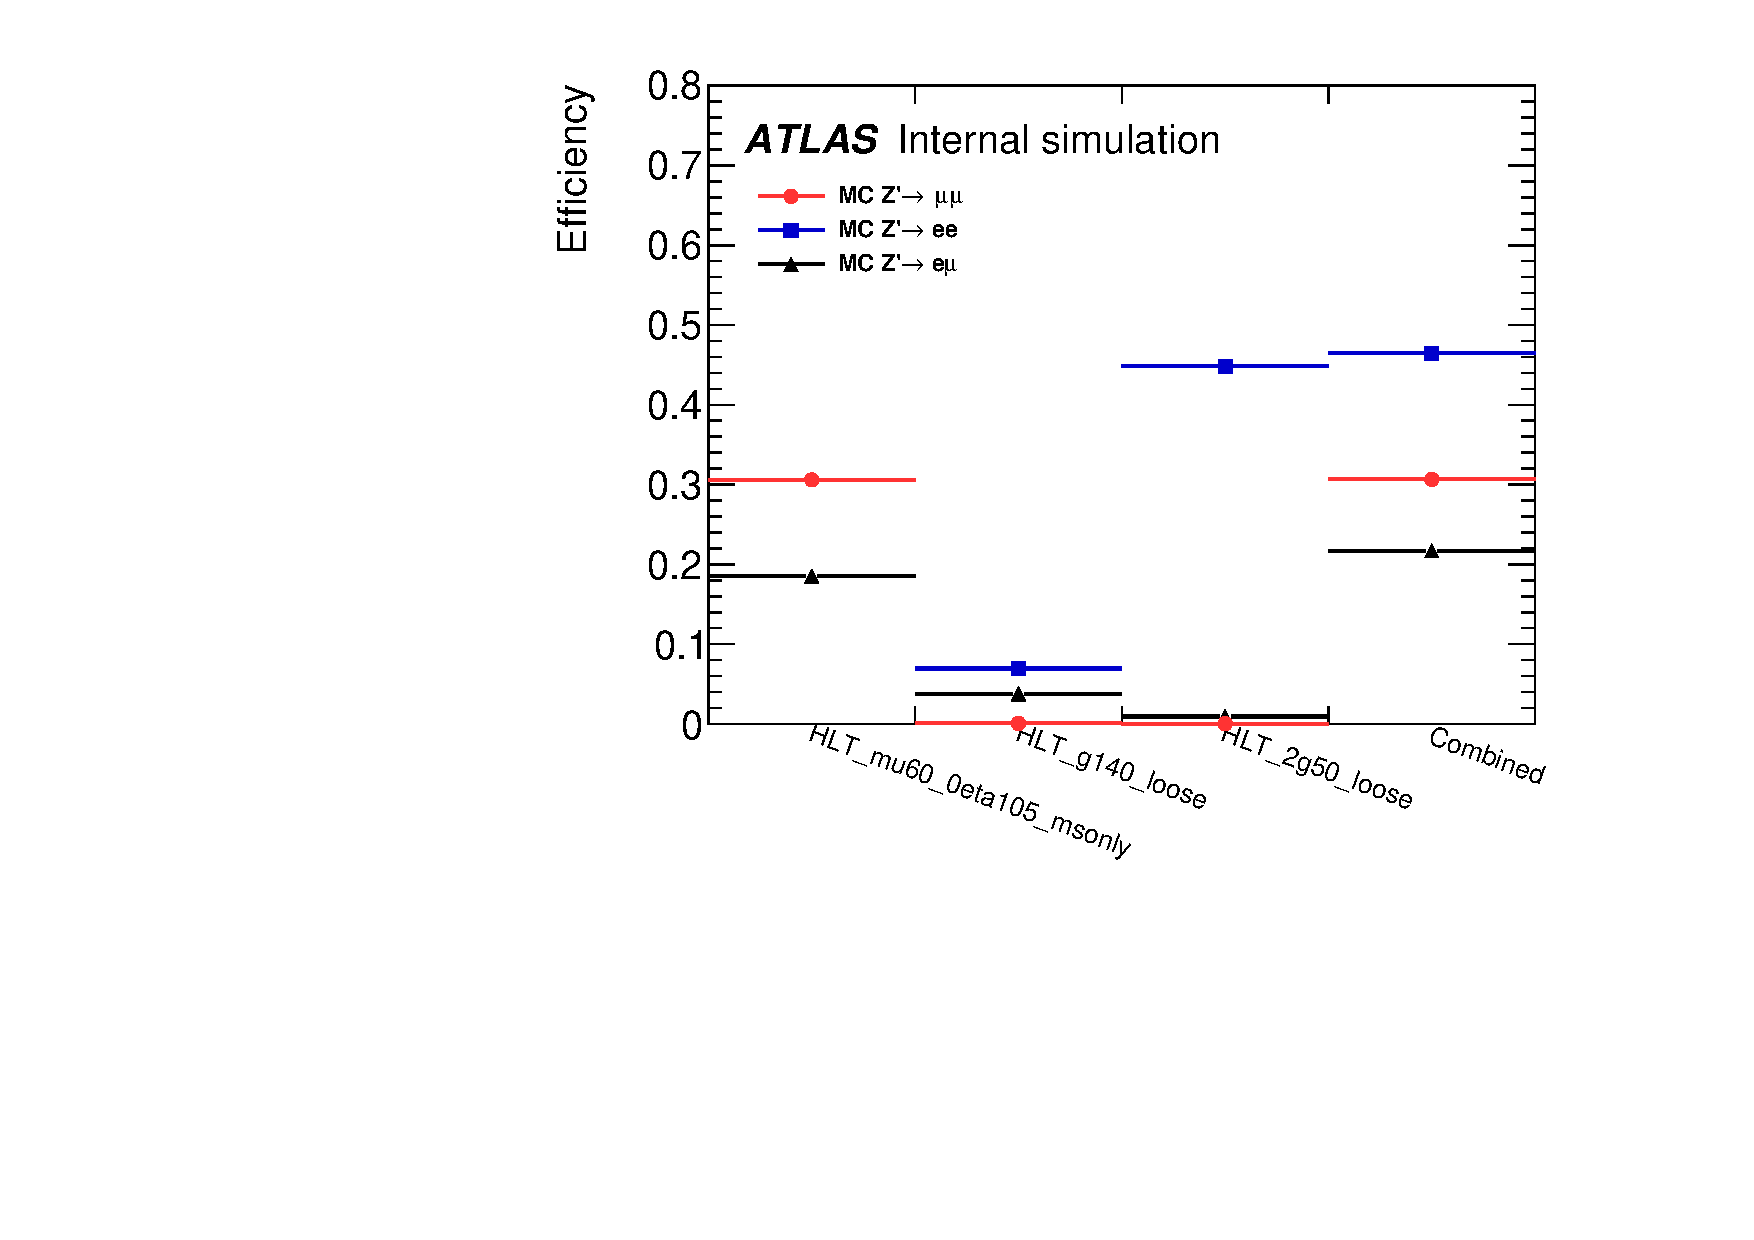
\includegraphics[width=0.50\textwidth]{figures/m_dv_eff_trig_allchannel.pdf}
	\centering
	\caption{Trigger efficiency of single muon, single photon, di-photon, and the combined triggers of the signal MC samples of $Z'\rightarrow\mumu, \ee$, and \emu generated with $m=$ 250 GeV and $c\tau=$ 250 mm.}
	\label{fig:m_trig_eff_allchannel}
\end{figure}

The trigger efficiency on all \mumu signal MC samples is shown in Table~\ref{table:m_trig_eff_mumu}. It is evident that at low $Z'$ mass ($\backsim$100 GeV), the combined trigger efficiency on the signal MC sample is significantly reduced because the typical $p_{T}$ of the signal muons is lower than the $p_{T}$ threshold of the single muon trigger.

The trigger study indicates that there is a substantial loss in the signal efficiency at trigger level before reconstruction, and developing dedicated, more efficient triggers for long-lived particles will provide potential improvement in sensitivity to long-lived particles. The systematic uncertainties in trigger efficiency is estimated by tag-and-probe method in Section~\ref{sec:syst:trigger}.

\begin{table}[!htb]
  \centering
  \begin{tabular}{ c c | c c c c}
    \hline
    \hline
    %       &       & \multicolumn{4}{c}{$Z'\rightarrow\mumu$}                \\
    $m_{Z'}$ (GeV) & $c\tau$ (mm) & Single muon & Single photon & Di-photon & Combined \\
    \hline
    100			&	100	& 0.047 	& < 0.001   &0  	    &0.047  		\\
    100			&	250	& 0.043  	&0  	 	&0  	    &0.043  		\\
    100			&	500	& 0.039 	&0  	 	&0  	    &0.039  		\\
    250			&	100	& 0.343  	&< 0.001 	&< 0.001    &0.344  		\\
    250			&	250	& 0.306  	&< 0.001 	&< 0.001    &0.307  		\\
    250			&	500	& 0.230 	&< 0.001 	&< 0.001    &0.230  		\\
    500			&	100	& 0.454 	&0.010   	&< 0.001    &0.459  		\\
    500			&	250	& 0.410 	&0.009   	&< 0.001    &0.415  		\\
    500			&	500	& 0.331  	&0.008   	&0.001      &0.336  		\\
    750			&	100	& 0.541 	&0.026   	&0.002      &0.553  		\\
    750			&	250	& 0.470 	&0.023   	&0.003      &0.481  		\\
    750			&	500	& 0.391 	&0.022 	    &0.001      &0.402  		\\
    1000	    &	100	& 0.570   	&0.039   	&0.004      &0.586  		\\
    1000	    &	250	& 0.512   	&0.036   	&0.003      &0.526  		\\
    1000	    &	500	& 0.430   	&0.034 	    &0.004      &0.444  		\\
    \hline
    \hline
  \end{tabular}
  \caption{Trigger efficiency of single muon, single photon, di-photon triggers, and the combined trigger efficiency on the signal MC samples of $Z'\rightarrow\mumu$.}
  \label{table:m_trig_eff_mumu}
\end{table}

\section{Lepton reconstruction efficiency}
\label{sec:tracking_efficiency}
The tracking efficiency, $\varepsilon_{\mathrm{track}}$, and the lepton identification efficiency, $\varepsilon_{\mathrm{lepton}}$, are studied together as a lepton reconstruction efficiency. The lepton reconstruction efficiency is defined and estimated as follows. From a signal MC sample, the leptons decaying from $Z'$ are collected at generator-level, referred as \textit{truth} signal leptons. For each truth signal lepton, if there is a reconstructed lepton with its ID track matched to the ID track of the truth signal lepton by a hit-based truth matching scheme, it is marked as reconstructed. The ratio of reconstructed signal leptons to the total number of signal leptons produced in the sample is taken as the lepton reconstruction efficiency. No \texttt{RPVLL} or trigger filter is applied in estimating the lepton reconstruction efficiency.

Figure~\ref{fig:lepton_eff} shows the representative plot of the lepton reconstruction efficiency as a function of track parameters using the combined signal MC samples of $Z'$ decaying to all three channels, generated with $m = $ 250 GeV and $c\tau=$ 250 mm.

\begin{figure}[!htb]
    \centering
    \subfloat[]{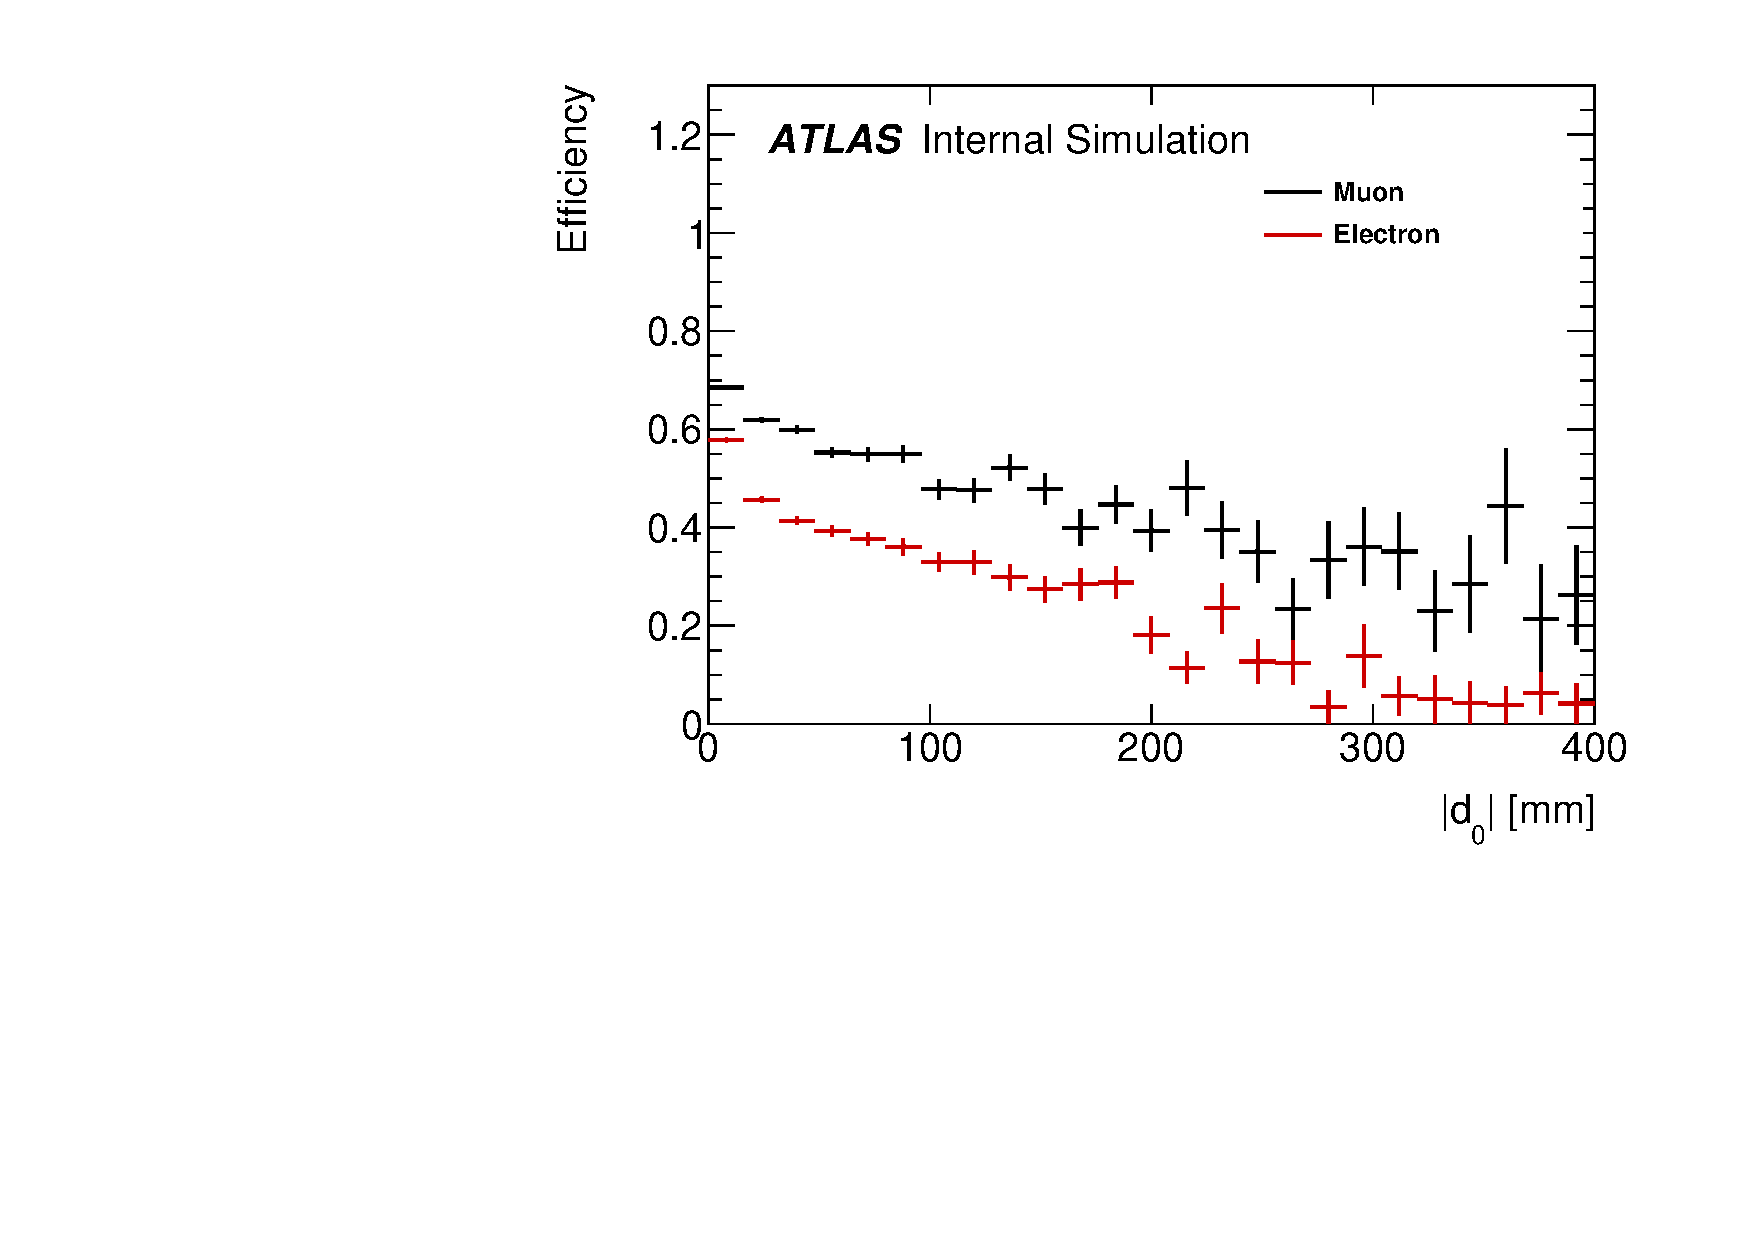
\includegraphics[width=0.50\textwidth]{figures/m_lepton_efficiency_d0.pdf}}
    \subfloat[]{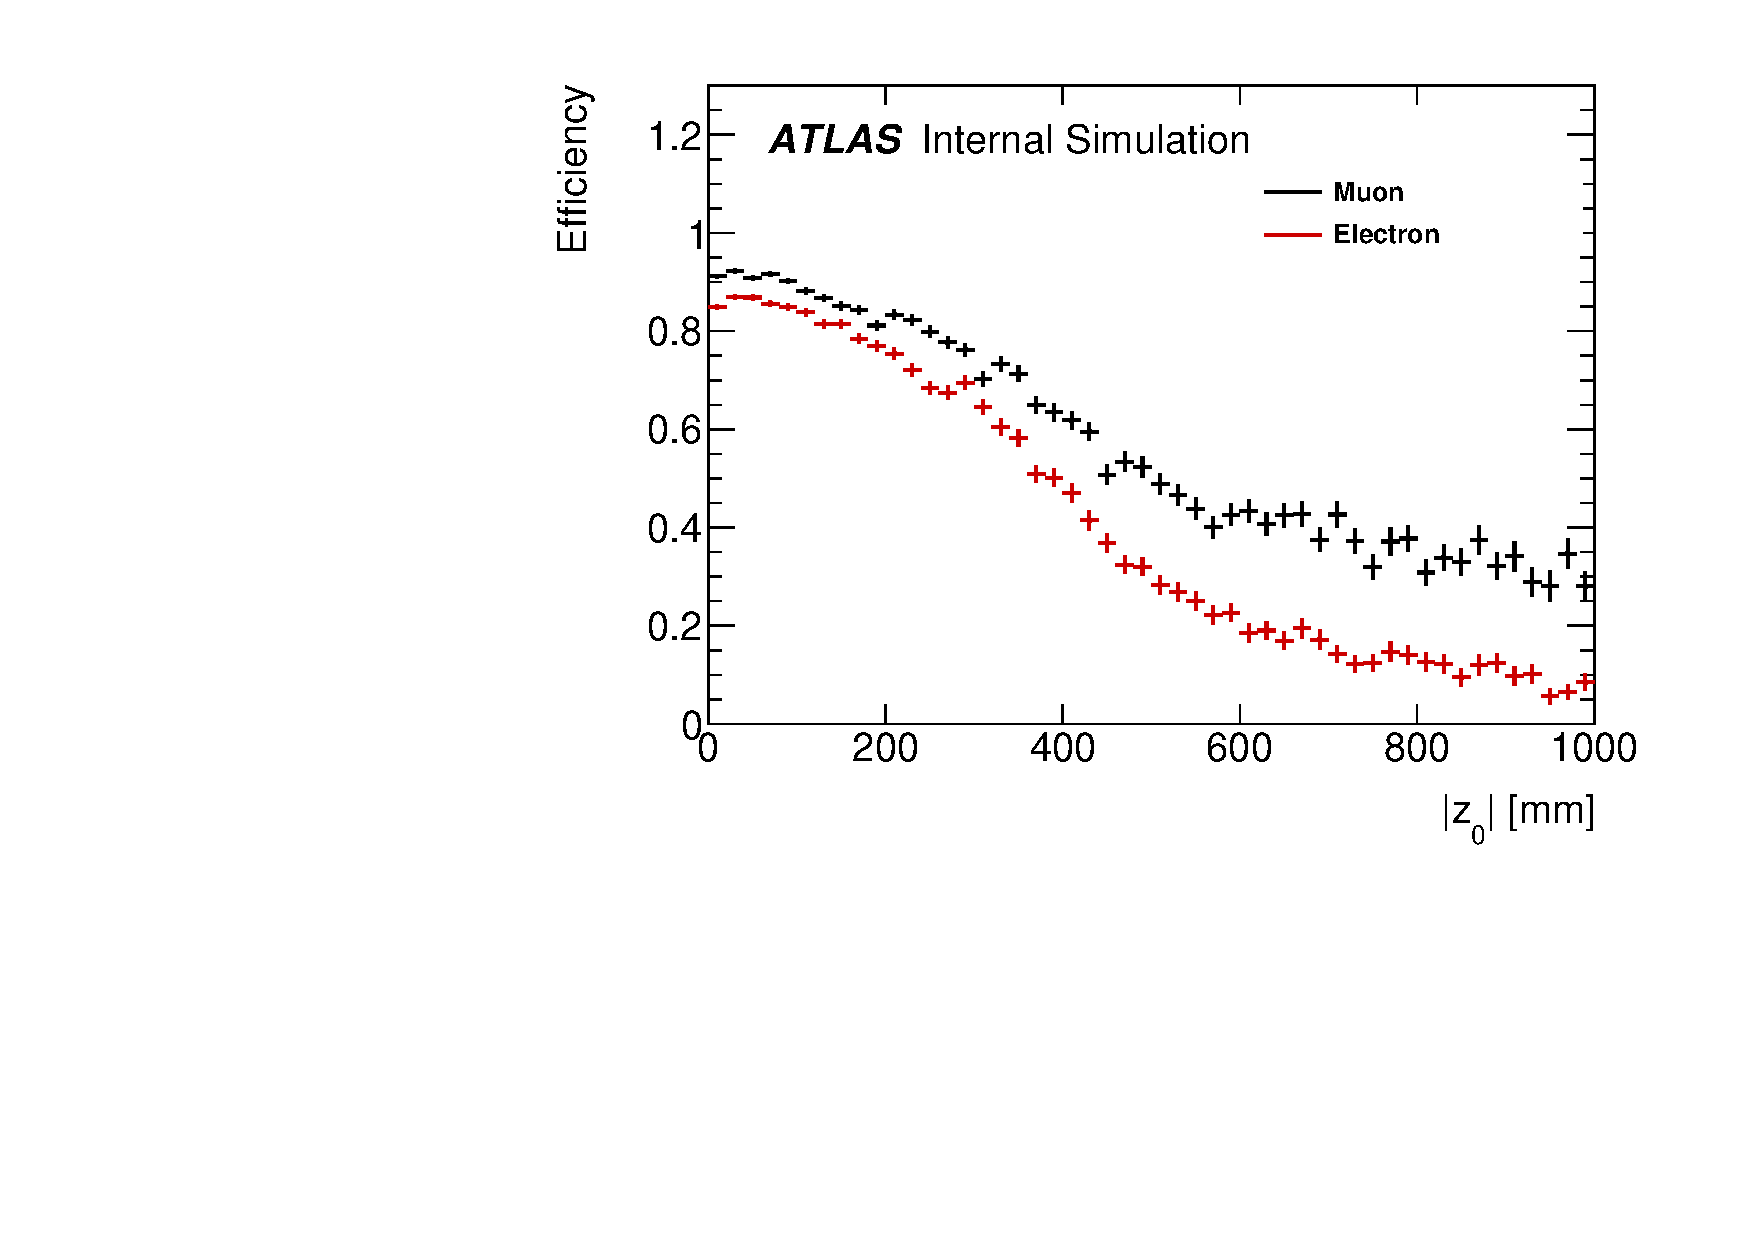
\includegraphics[width=0.50\textwidth]{figures/m_lepton_efficiency_z0.pdf}} \\
    \subfloat[]{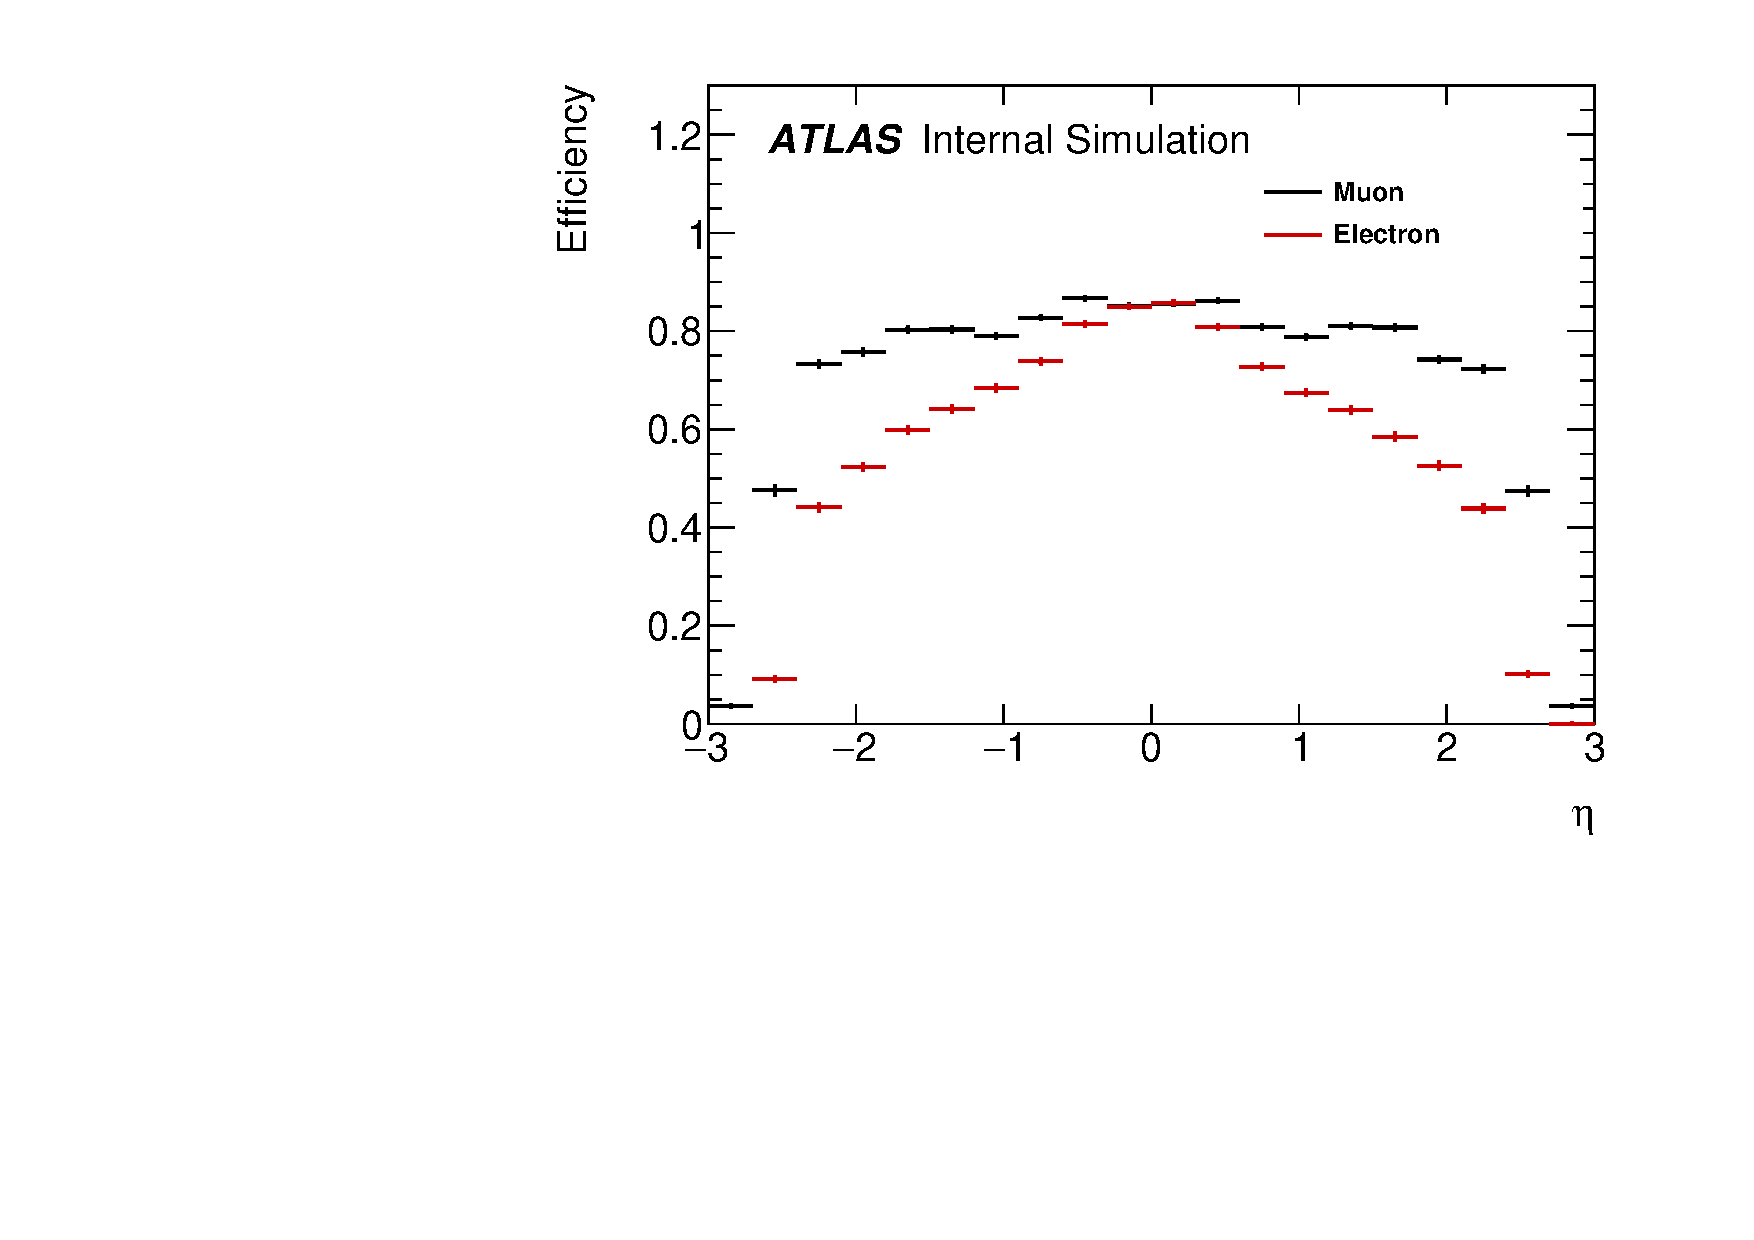
\includegraphics[width=0.50\textwidth]{figures/m_lepton_efficiency_eta.pdf}}
    \subfloat[]{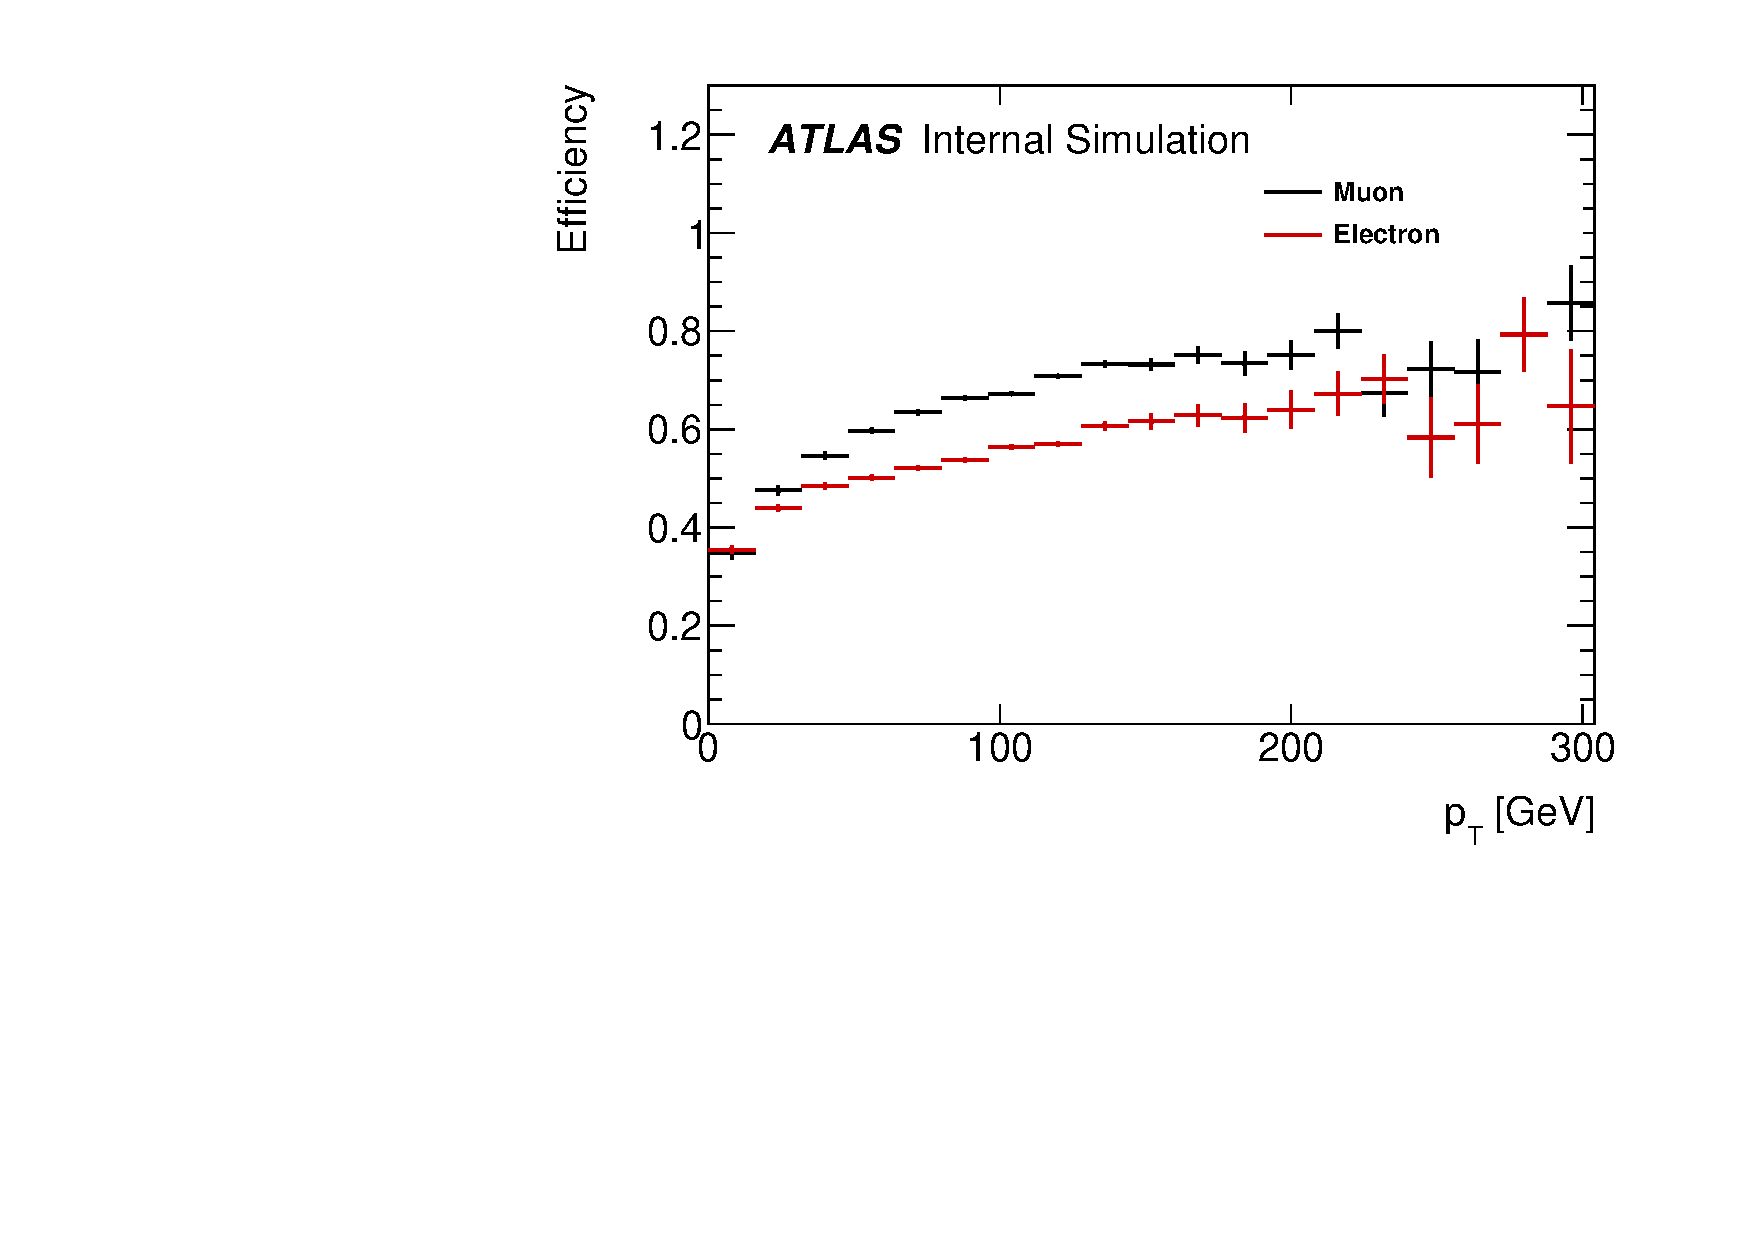
\includegraphics[width=0.50\textwidth]{figures/m_lepton_efficiency_pt.pdf}} 
    \caption{Lepton reconstruction efficiency as a function of (a) $d_{0}$, (b) $z_{0}$, (c) $\eta$, and (d) $p_{T}$ of signal leptons using the signal MC sample generated with $m=$ 250 GeV and $c\tau=$ 250 mm.}
    \label{fig:lepton_eff}
\end{figure}

It is evident that the efficiency drops drastically at $\eta > 2.0$ where the Pixel barrel region ends due to the minimum silicon hits requirement on tracks as shown in Table~\ref{table:tracking}. The efficiency is not very sensitive to $p_{T}$ except low $p_{T}$ region ($p_{T} < 20$).

The lepton reconstruction efficiency decreases for large $d_{0}$ and $z_{0}$. In the signal MC samples, most of $Z'$ decay within the Pixel barrel region, $r < $ 122.5 mm and $z < $ 400.5 mm, where the lepton reconstruction efficiency is high.

\section{Overall reconstruction efficiency}
\label{sec:combined_reco_efficiency}
The overall reconstruction efficiency is defined as the ratio of $Z'$s reconstructed as displaced vertices in the signal region to the total $Z'$ produced in the sample. In this section, representative plots of event cut flow, vertex cut flow (Section~\ref{sec:signal_cutflow}), and overall reconstruction efficiency distributions (Section~\ref{sec:signal_vertex_distribution}) are presented using the signal MC samples generated with $m=$ 500, 1000 GeV, and $c\tau=$ 100 mm.

%In Section~\ref{sec:efficiency_reweighting}, the overall reconstruction efficiency is reweighted to reproduce pile-up distribution in the data sample. The reconstruction efficiency for all MC samples is also presented.


\subsection{Event and vertex cut flow}
\label{sec:signal_cutflow}
The MC samples are processed with steps described in Section~\ref{sec:selection:pre}. The analysis-level cuts, the event and the vertex selections described in Table~\ref{table:signal_selection}, are applied to the processed samples. Representative plots of the event cut flow and the vertex cut flow are shown in Figure~\ref{fig:signal_cutflow_MC_mumu} using the signal MC samples of $Z'$ decaying to \mumu generated with $m=$ 500, 1000 GeV for $c\tau=$ 100 mm.

\begin{figure}[!htb]
    \centering
    \subfloat[]{\label{subfig:event_cutflow_MC}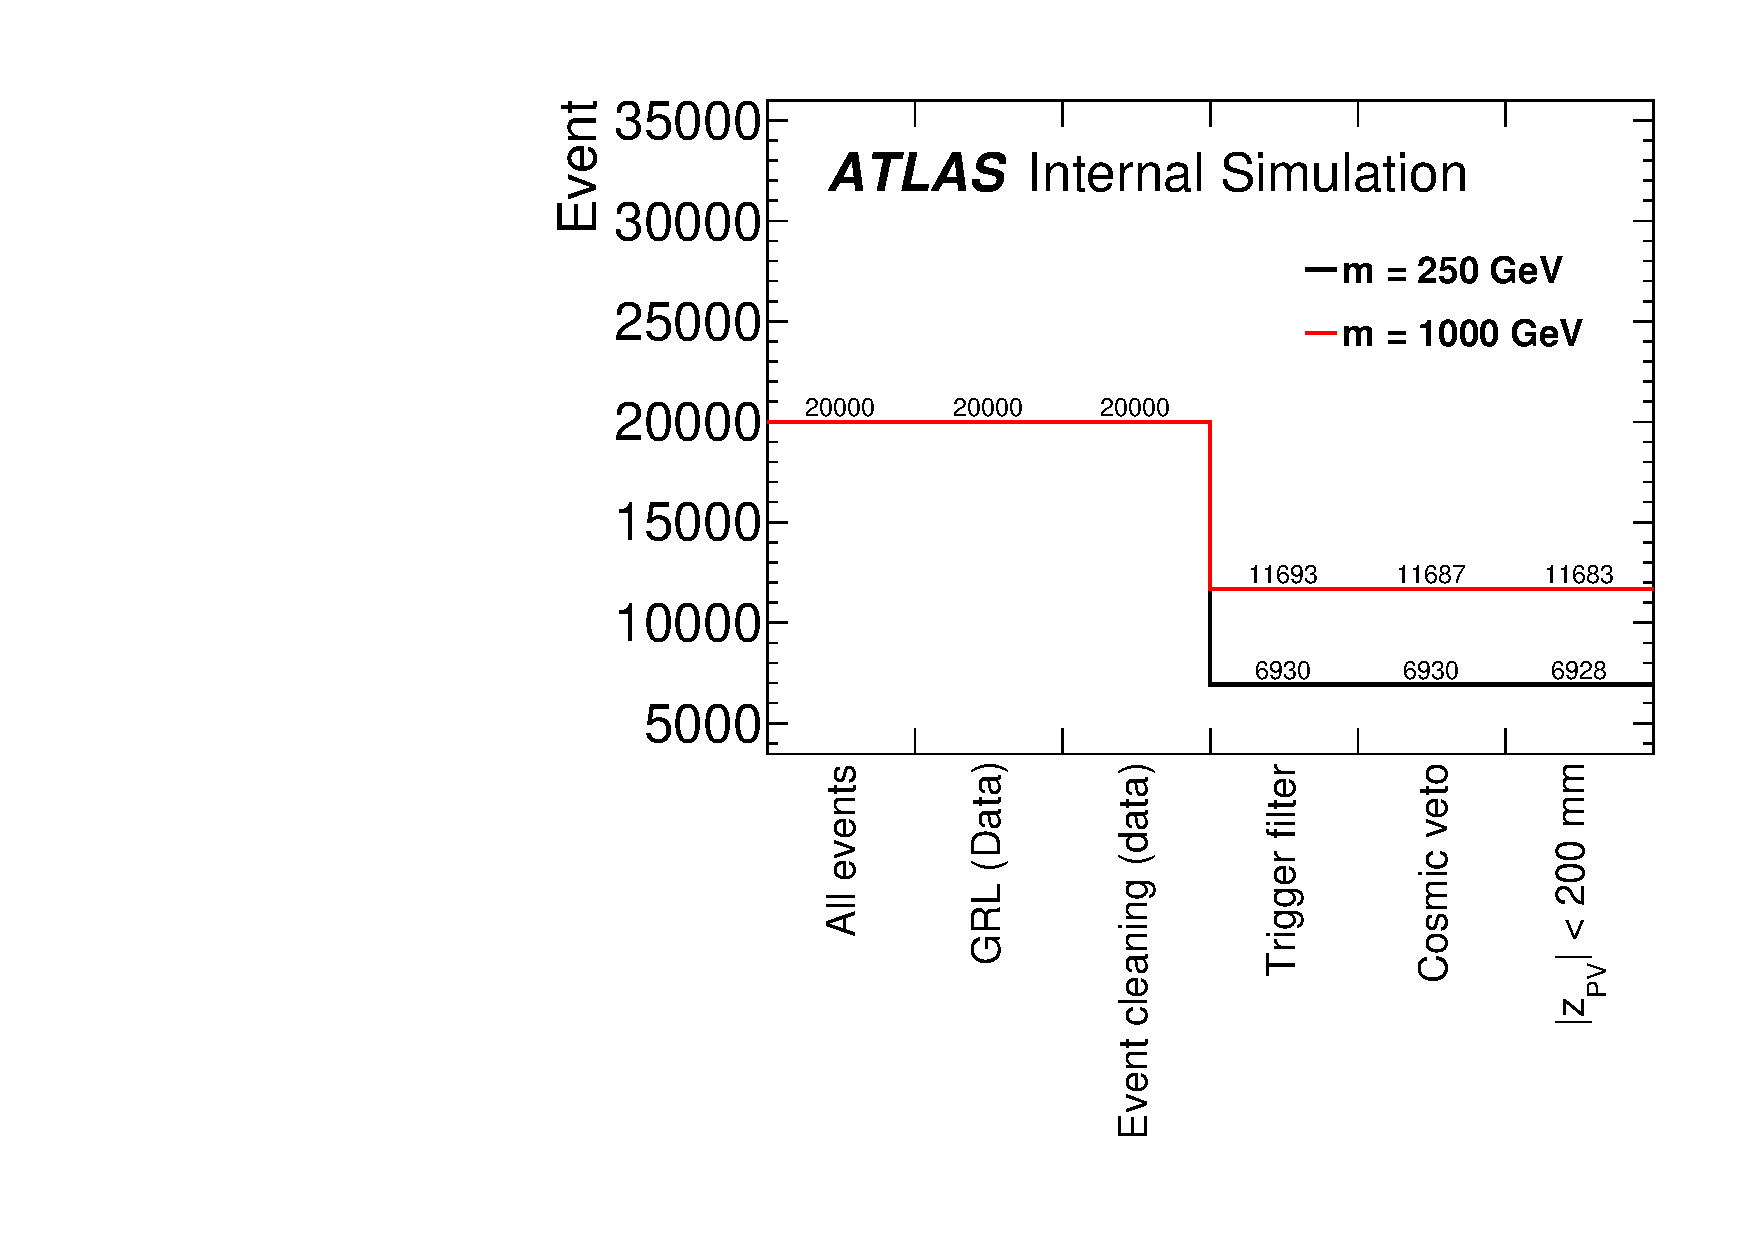
\includegraphics[width=0.50\textwidth]{figures/m_event_cutflow_MC_mumu.pdf}}
    \subfloat[] {\label{subfig:vertex_cutflow_MC}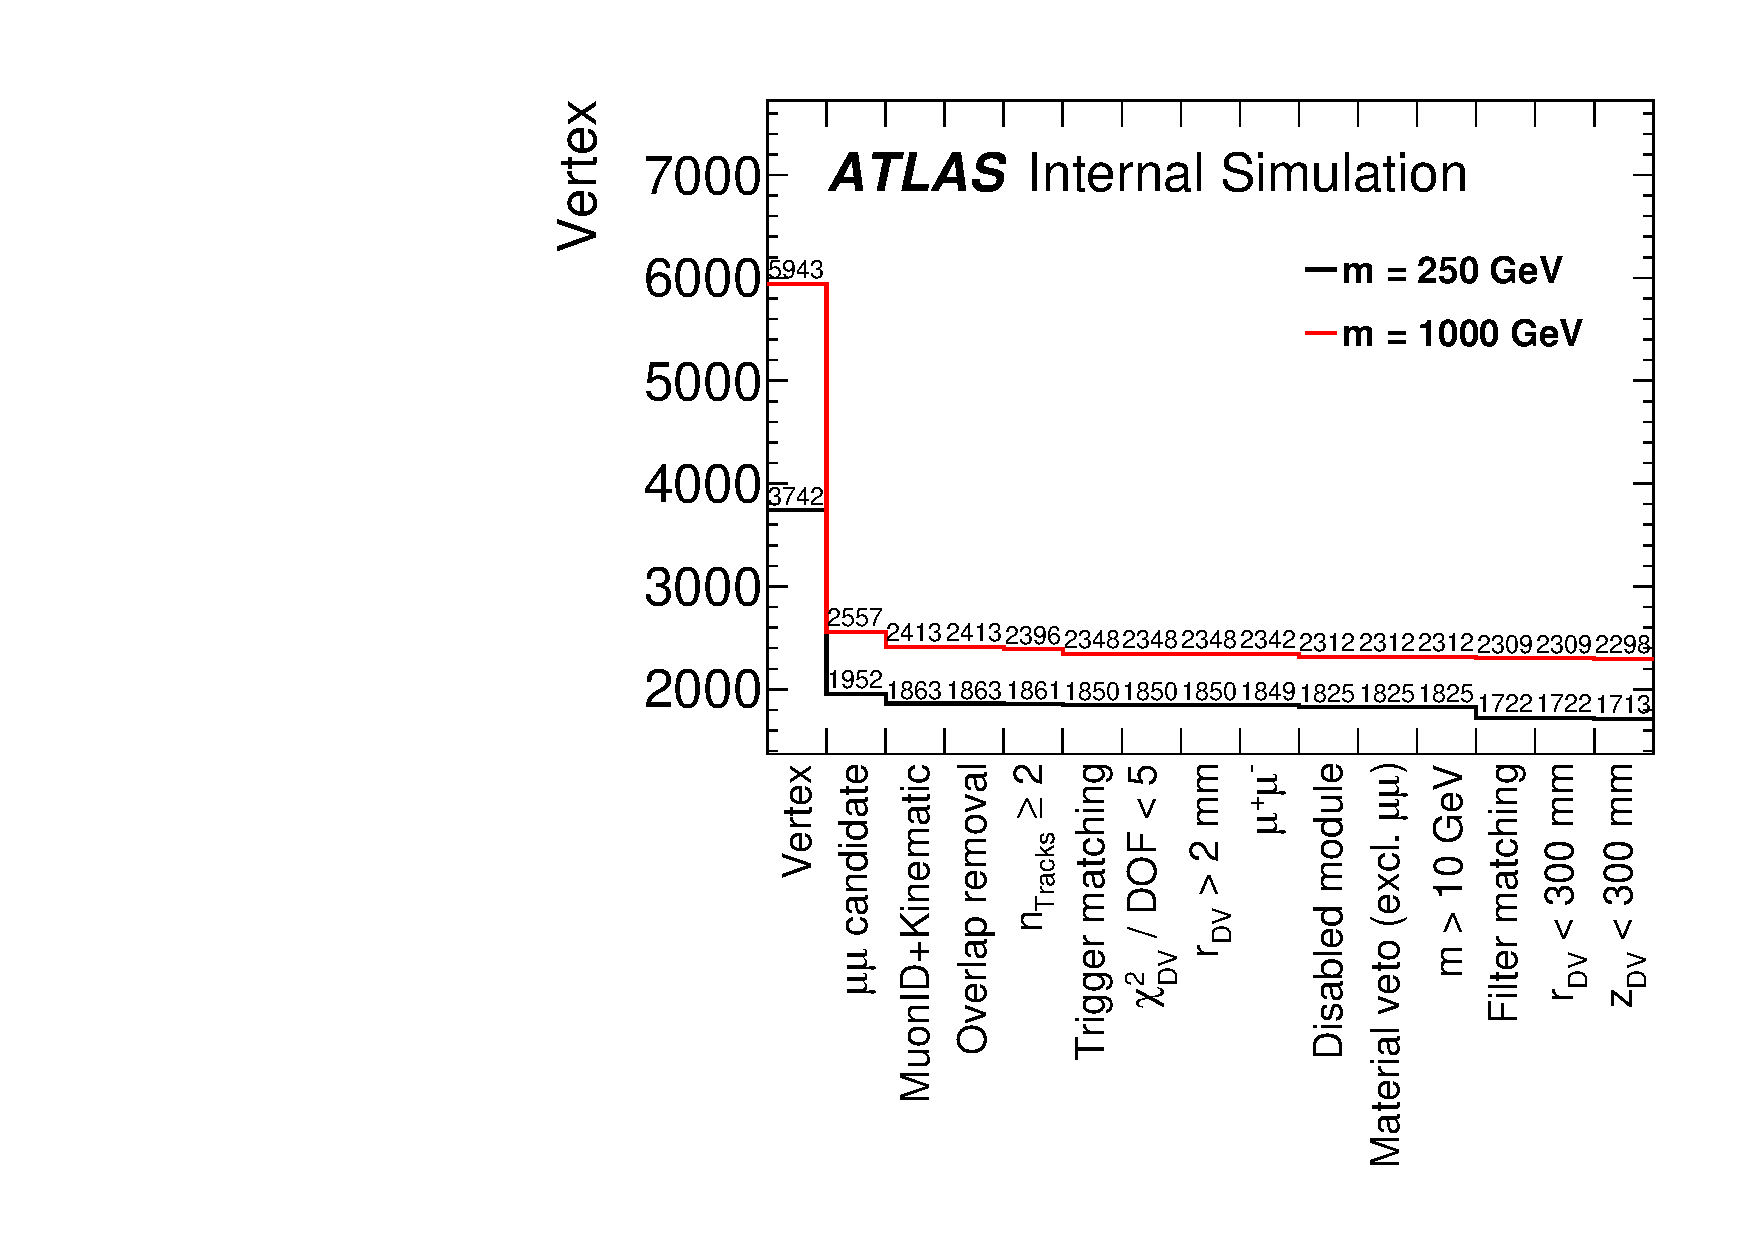
\includegraphics[width=0.50\textwidth]{figures/m_dv_cutflow_MC_mumu.pdf}} \\
    \caption{(a) Event cut flow, and (b) vertex cut flow using the signal MC samples of $Z'\rightarrow \mumu$ generated with $m =$ 500,1000 GeV for $c\tau= $ 100 mm.}
    \label{fig:signal_cutflow_MC_mumu}
\end{figure}

In the event cut flow, \texttt{RPVLL} filter is applied during the sample processing. \texttt{GoodRunsList} filter and Event cleaning are shown as place holders as they are only applied to data sample.

In the vertex cut flow, displaced vertices are reconstructed in about $\backsim$25$\%$ of the signal events passing the event selection, indicating that there is a significant loss of signal efficiency in the reconstruction process. The following selection criteria, $\chi^{2} /$ DOF $<$ 5 and the minimum displacement cut ($r > $ 2 mm), are applied, but the effect is expected to be very small as the same requirements are applied in the secondary vertex reconstruction algorithm. Material veto is applied to all vertex types except \mumu vertex. The minimum dilepton mass requirement and cosmic veto cuts have minimum impact on the signal efficiency.

\subsection{Efficiency distribution}
\label{sec:signal_vertex_distribution}
The overall reconstruction efficiency is studied by examining the efficiency distributions in the transverse ($r$), longitudinal ($z$) vertex position, and the angular distributions of the reconstructed vertices. The representative efficiency distributions are shown in Figure~\ref{fig:signal_vertex_dist} using the signal MC samples generated with $m =$500, 1000 GeV for $c\tau=$100 mm.

The overall efficiency shows a significant dependence on vertex position which decreases at large $r$ and $z$ due to the minimum silicon hits requirement on tracks. The first bins in $r$ and $z$ distributions have lower efficiency due to the minimum displacement requirement ($r > $ 2 mm) on secondary vertices. The $r$ distribution shows features that reflects the physical structure of the ID. The $\eta$ distribution has higher efficiency in the central region, and the $\phi$ distribution is uniform as expected.


\begin{figure}[!htb]
    \centering
    \subfloat[]{\label{subfig:vertex_dist_r  }\includegraphics[width=0.50\textwidth]{figures/m_dv_efficiency_r.pdf}}
    \subfloat[]{\label{subfig:vertex_dist_z  }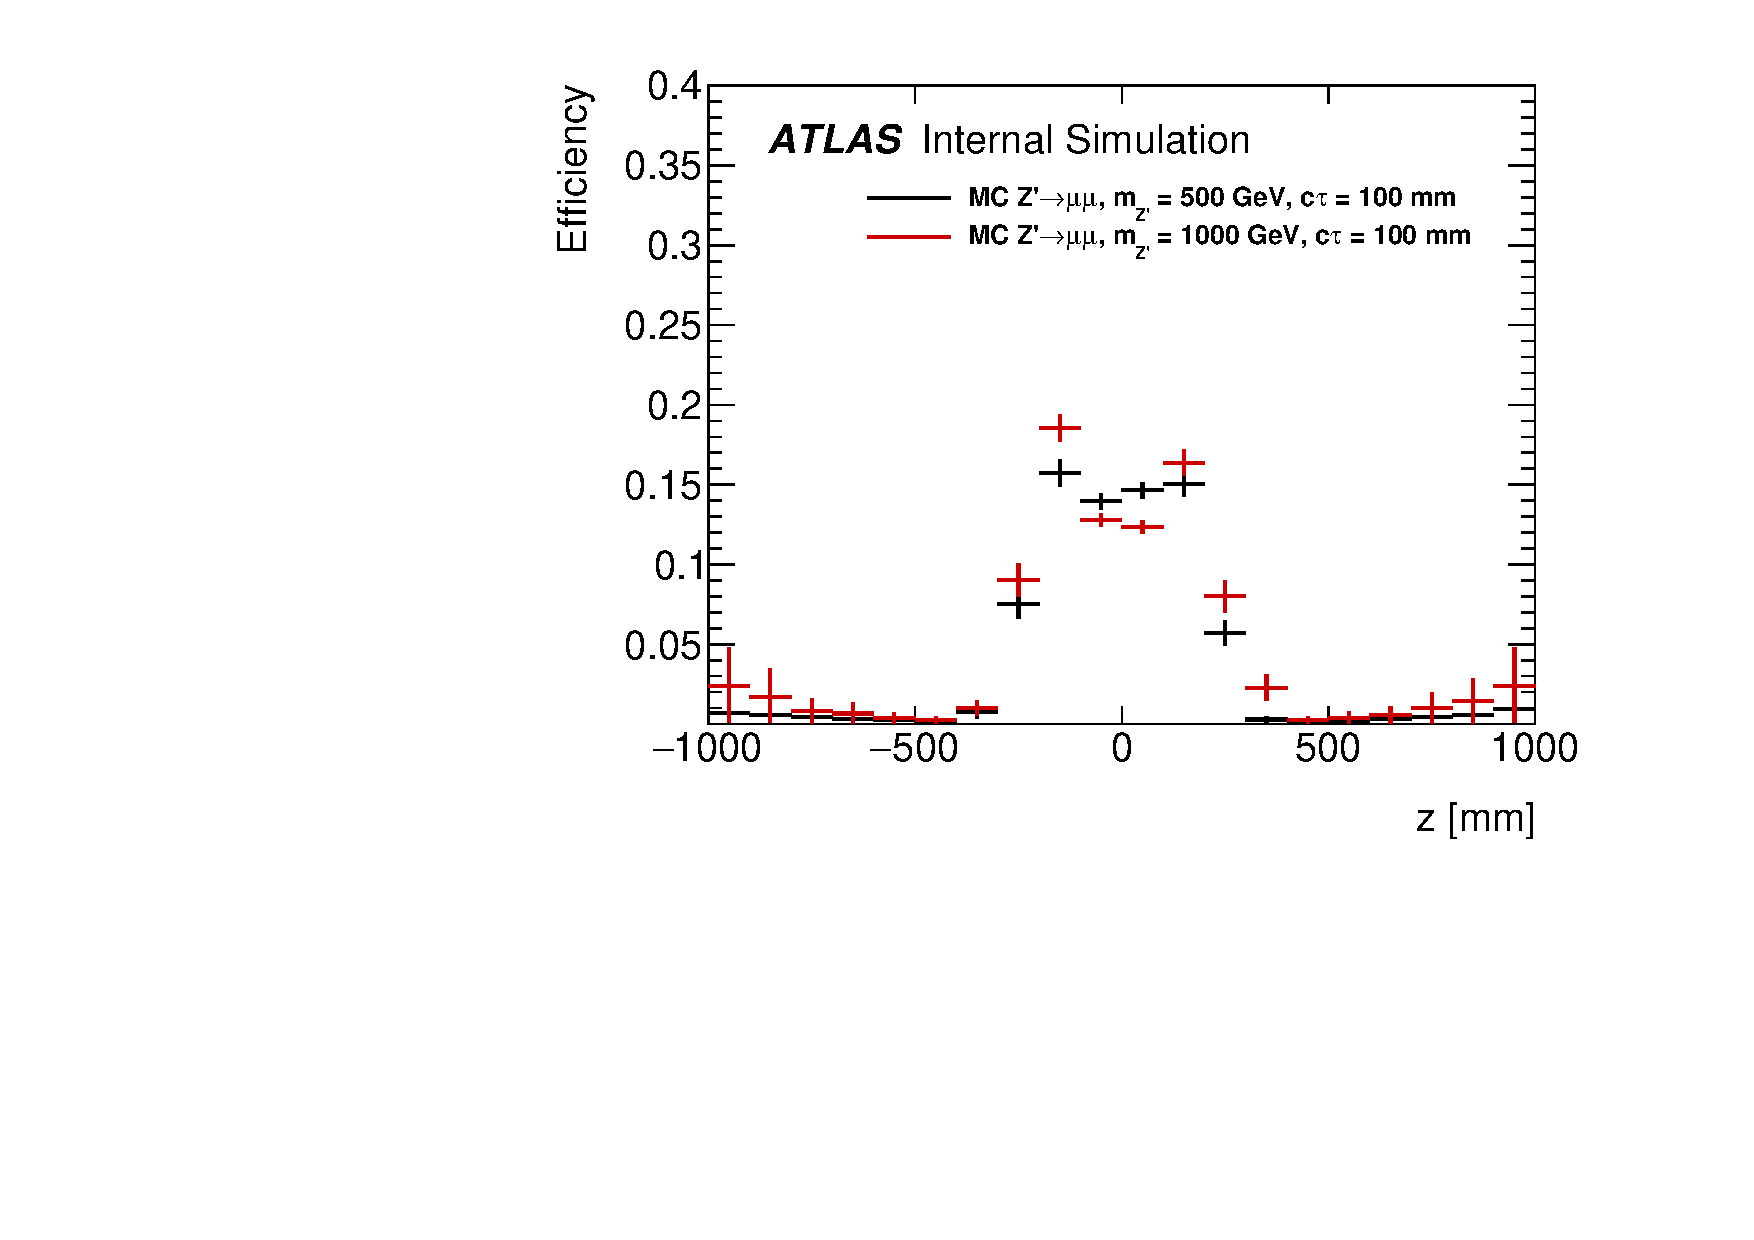
\includegraphics[width=0.50\textwidth]{figures/m_dv_efficiency_z.pdf}} \\
    \subfloat[]{\label{subfig:vertex_dist_eta}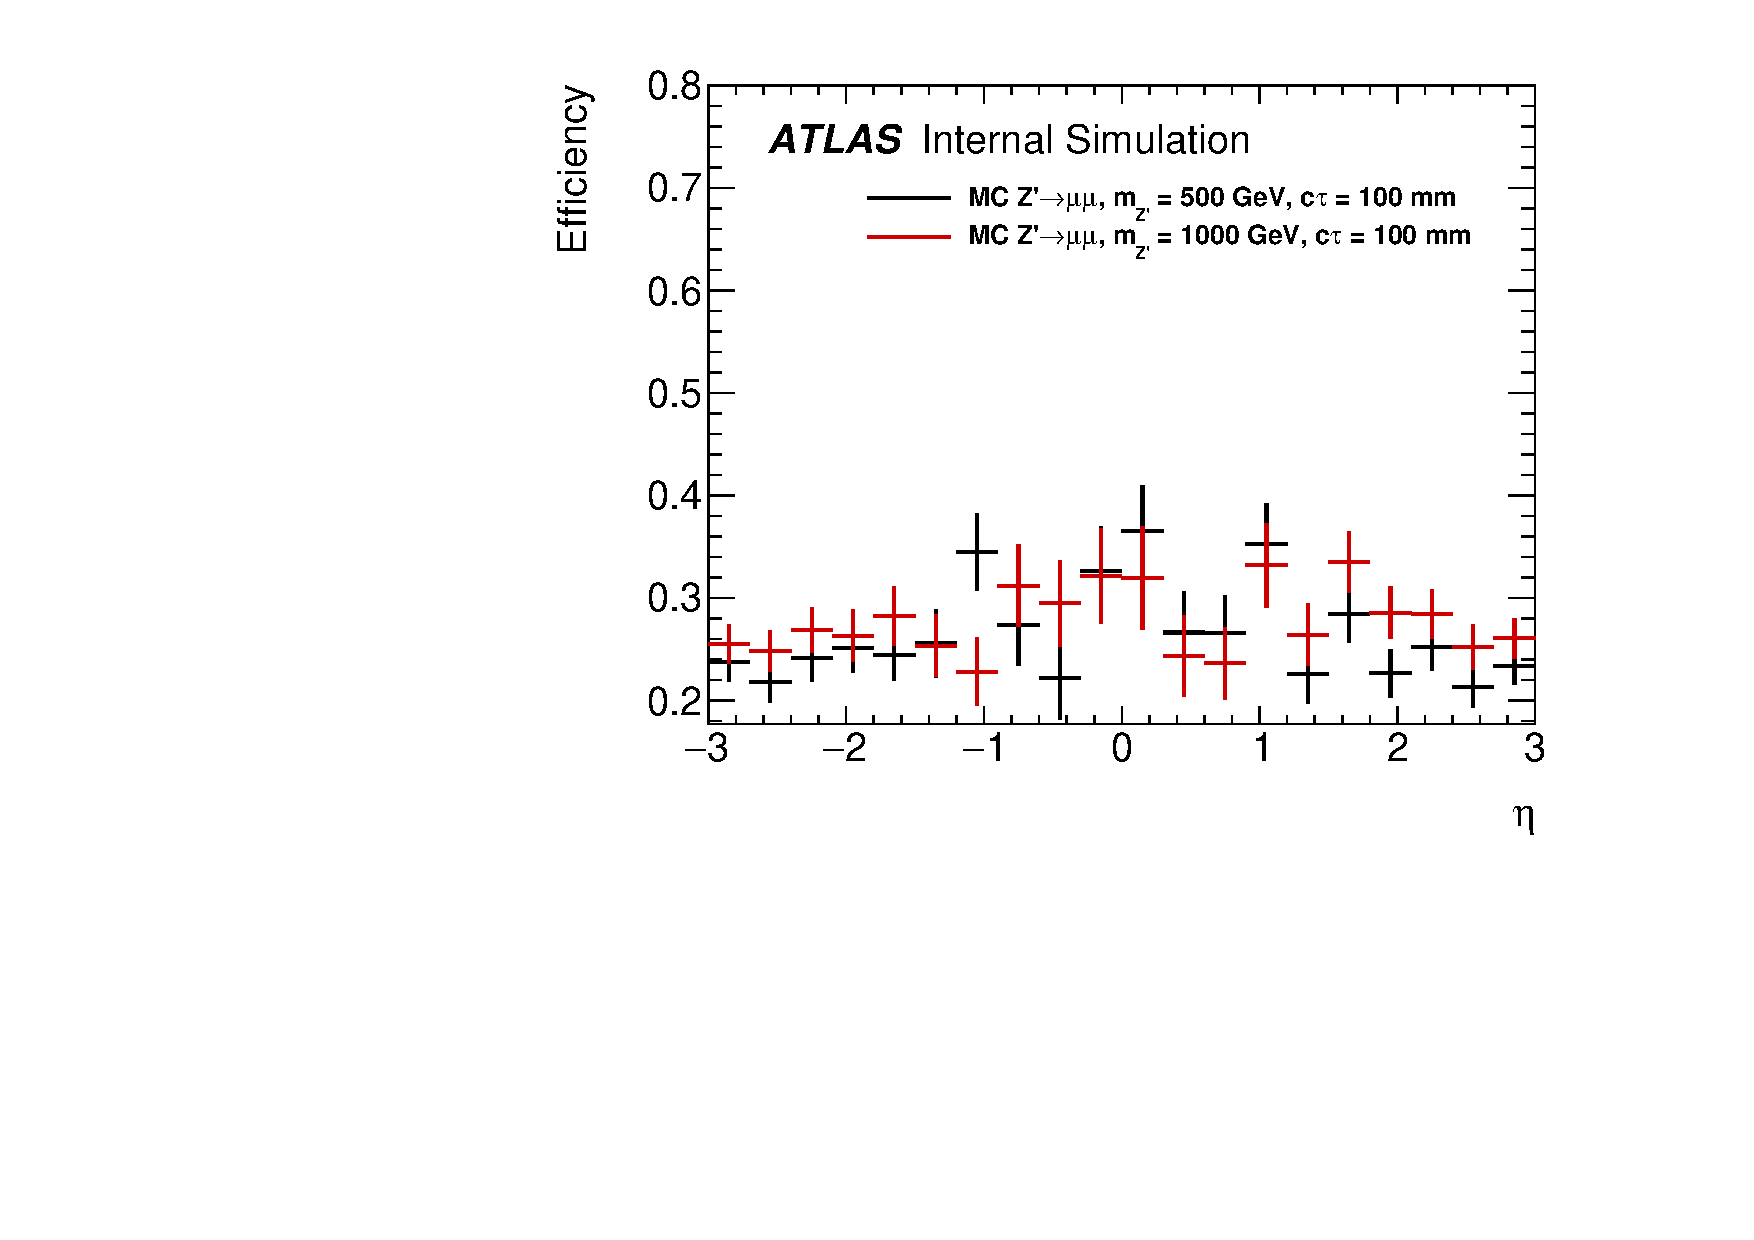
\includegraphics[width=0.50\textwidth]{figures/m_dv_efficiency_eta.pdf}}
    \subfloat[]{\label{subfig:vertex_dist_phi}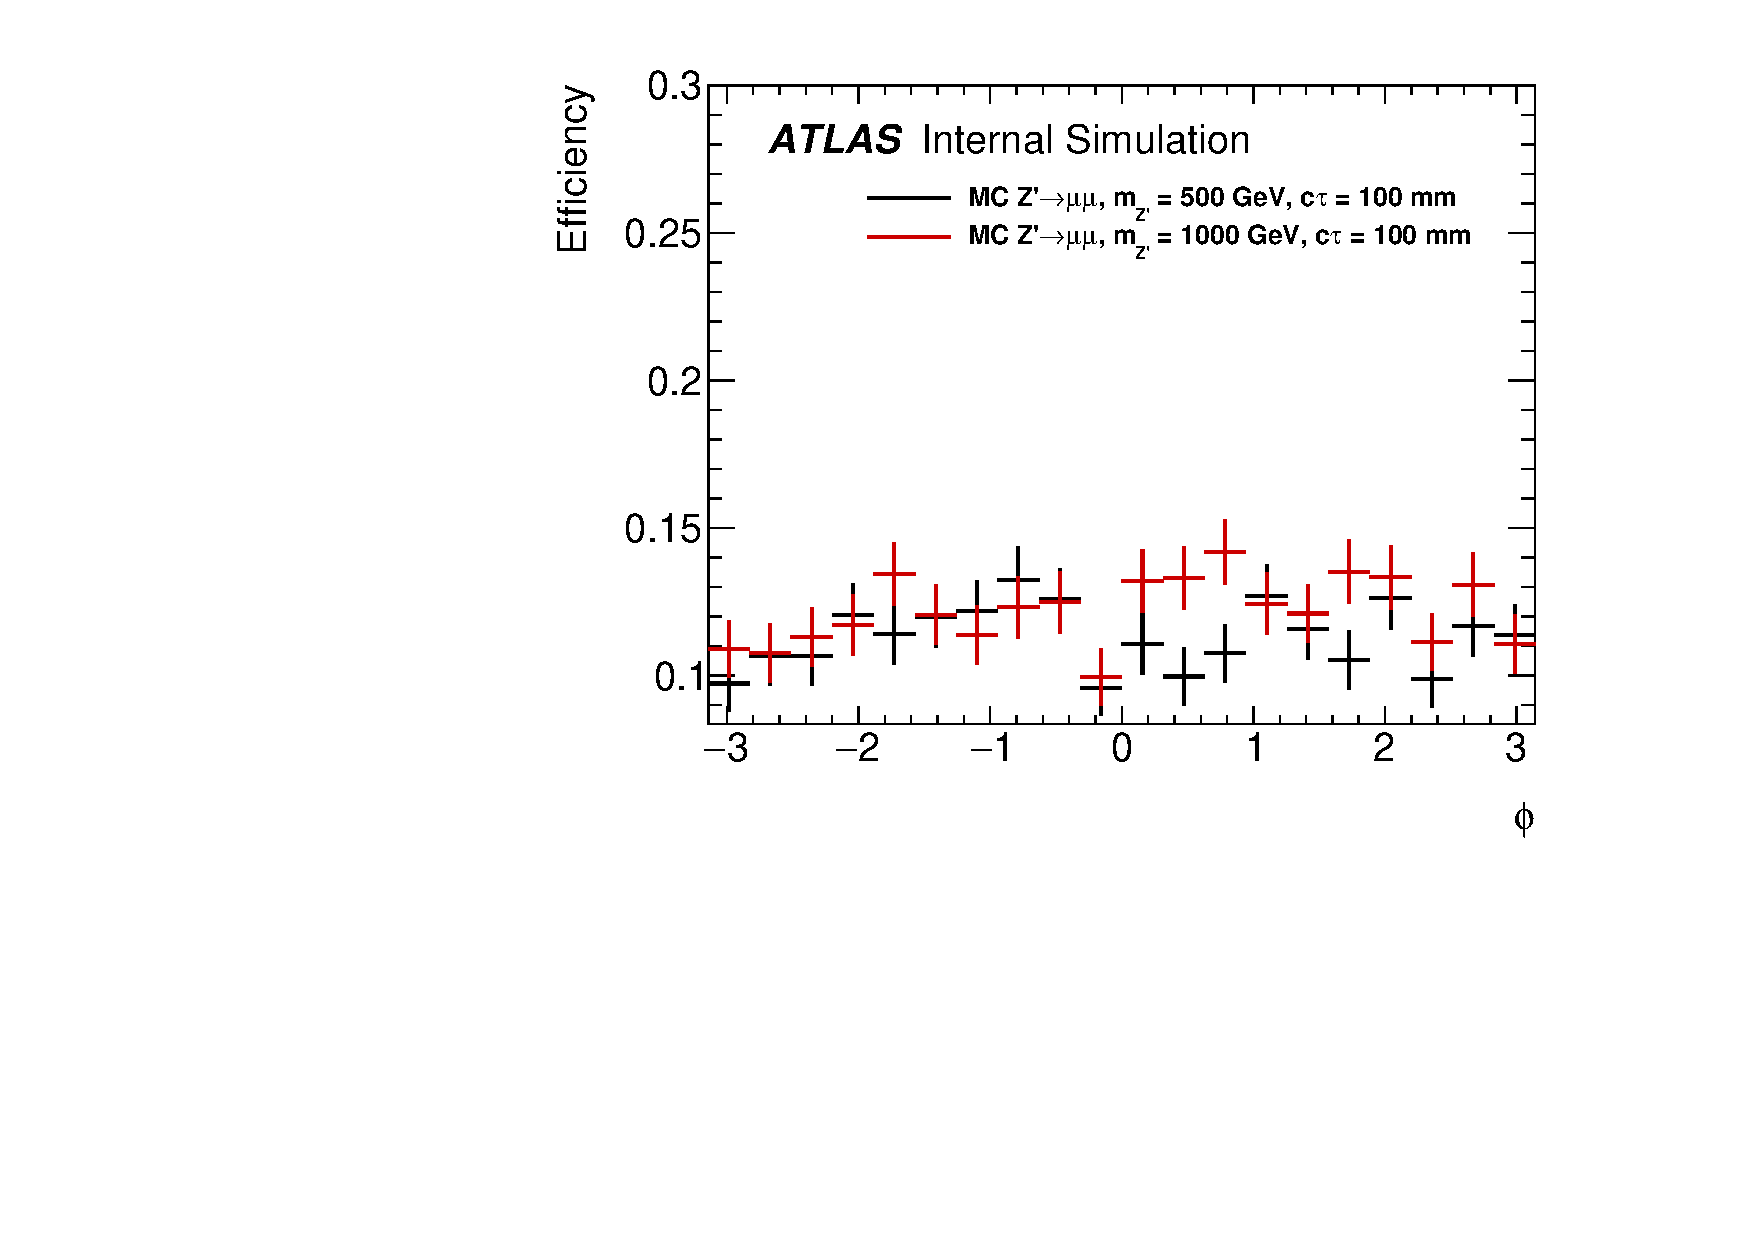
\includegraphics[width=0.50\textwidth]{figures/m_dv_efficiency_phi.pdf}} 
    \caption{Overall efficiency distributions in (a) $r$, (b) $z$, (c) $\eta$, and (d) $\phi$ of the signal MC samples of $Z'\rightarrow \mumu$ with $m=$ 500, 100 GeV for $c\tau=$ 100 mm.}
    \label{fig:signal_vertex_dist}
\end{figure}





%\begin{table}[!htb]
%  \centering
%  \begin{tabular}{ c c | c c  }
%    \hline
%           &       & \multicolumn{2}{c}{$Z'\rightarrow\mumu$}                \\
%    $m_{Z'}$ (GeV) & $c\tau$ (mm) & unweighted & reweighted \\
%    \hline
%    100			&	100	& 0.0472$\pm$0.0026 	&0.0593$\pm$0.0033  \\
%    100			&	250	& 0.0323$\pm$0.0021 	&0.0399$\pm$0.0028 	\\
%    100			&	500	& 0.0184$\pm$0.0016		&0.0243$\pm$0.0023 	\\
%    250			&	100	& 0.2010$\pm$0.0049		&0.2200$\pm$0.0058	\\
%    250			&	250	& 0.1759$\pm$0.0046 	&0.1848$\pm$0.0053	\\
%    250			&	500	& 0.1315$\pm$0.0042		&0.1375$\pm$0.0048	\\
%    500			&	100	& 0.2284$\pm$0.0053		&0.2473$\pm$0.0062	\\
%    500			&	250	& 0.2001$\pm$0.0049		&0.2083$\pm$0.0056	\\
%    500			&	500	& 0.1554$\pm$0.0045 	&0.1629$\pm$0.0052 	\\
%    750			&	100	& 0.2340$\pm$0.0052		&0.2485$\pm$0.0060 	\\
%    750			&	250	& 0.2277$\pm$0.0051		&0.2341$\pm$0.0058 	\\
%    750			&	500	& 0.1654$\pm$0.0045		&0.1670$\pm$0.0050  \\
%    1000	    &	100	& 0.2253$\pm$0.0051 	&0.2421$\pm$0.0059 	\\
%    1000	    &	250	& 0.2301$\pm$0.0050 	&0.2337$\pm$0.0057	\\
%    1000	    &	500	& 0.1871$\pm$0.0047  	&0.1854$\pm$0.0052  \\
%    \hline
%  \end{tabular}
%  \caption{}
%  \label{table:m_signal_eff_mumu_all}
%\end{table}





%TABLE SHOWING ALL EFFICIENCY GOES HERE
